\documentclass[journal]{IEEEtran}

\usepackage{cite}
\usepackage{authblk}
\usepackage[pdftex]{graphicx}
\usepackage{amsmath}
\usepackage{algorithmic}
\usepackage{array}
\usepackage{url}

% correct bad hyphenation here
\hyphenation{op-tical net-works semi-conduc-tor}

\begin{document}

% paper title
\title{Proposal: Enhanced Movie Searching and Recommendations with LLM’s}

% author names and affiliations
\author[1]{Micah Keith Harlan}
\author[1]{Jianger Yu}
\author[1]{Baiyi Zhang}

% For affiliations, directly adjust the font size using \small, \footnotesize, etc.
\affil[1]{{\small \{mharlan25, jianger, baiyi\}@vt.edu}}
\affil[1]{{\small Department of Computer Science, Virginia Polytechnic Institute and State University, Falls Church, VA, USA}}

% Make the title area
\maketitle

% abstract
\begin{abstract}
The rise of streaming services has revolutionized the way we consume media, offering an unprecedented volume of content at our fingertips. However, this abundance has led to a paradox of choice, where users often find themselves overwhelmed, scrolling through streaming platforms for extended periods without being able to decide on a movie to watch. Traditional search mechanisms in these platforms typically hinge on metadata such as movie titles, genres, and actor names, which, despite their utility, often need to catch up in catering to the nuanced preferences of users. By incorporating Large Language Models (LLMs), it can offer a more nuanced search capability, allowing users to find movies based on detailed aspects of the content, such as thematic elements, narrative style, or emotional tone, far beyond what conventional metadata can provide. This paper aims to provide an innovative way in regards to query and recommend movies to users, by providing an interactive application, where a user can query for, and get recommended movies to reduce user browsing time.
\end{abstract}

% Note that keywords are not normally used for peer-reviewed papers.
\begin{IEEEkeywords}
IEEE, journal, \LaTeX, paper, template.
\end{IEEEkeywords}

\section{Introduction}
% The very first letter is a 2-line initial drop letter followed by the rest of the first word in caps.
\IEEEPARstart{M}{ovie} streaming services have revolutionized the way we consume entertainment, offering users the power of choice and flexibility. Users can watch virtually anything they want anytime they want. Streaming services have provided many advantages for the user, but with these advantages come challenges. 

Users have been faced with an overabundance of movies and or content to choose from. Streaming services provide users with a plethora of options, but users often find themselves scrolling for long periods, without selecting content to watch. The challenge underscores the urgent need for a movie data search and recommendation system capable of providing information to the user’s query as well as providing better suggestions to both the query and individual user preferences. This project aims to create an effective system for movie recommendation, and querying that reduces a user's overall browsing time.

This project aims to build an innovative movie information retrieval (IR) and recommendation system. The methods to respond to users’ queries are: (1) searching specific information. For example, the title and cast of the movie; (2) providing generic movie recommendations using machine learning. The main tasks of the project includes retrieving data from both indexed databases and the Internet, providing Top-N movie recommendations for the search using ranking algorithms, and displaying the search results in a User Interface (UI). To ensure both usability and performance, the project will also involve pre-training the machine learning model for recommendation and utilizing large language models for enhancing query rewriting and summarizing search results, in addition to the primary tasks. 

\section{Related Works}
In this section, studies relating to Traditional Information Retrieval (IR) systems, systems based on machine learning, and the usage of LLMs are introduced for searching and making content recommendations.

\subsection{Traditional IR System}
Modern Information Retrieval\cite{RN15} includes the algorithms and mathematical tools to determine query-document relevance, the best practice for indexing and ranking the search results. Introduction to Information Retrieval\cite{manning2008introduction} introduces the machine learning models and algorithms from the natural language processing (NLP) perspective. Priya et al\cite{6508326} proposed an ontology-based semantic query suggestion for movie search. This work can be leveraged in suggesting alternatives to a user’s initial query. They translated the keyword-based query to an ontology-based and structured query. Haughton et al\cite{RN16} introduced the method to interact with IMDb’s basic database and to retrieve user reviews. 

\subsection{Recommendation System}
Many research articles have been published on the topic of movie recommendation, including several comprehensive surveys\cite{RN19}. These surveys primarily reviewed the filtering and the algorithms for this topic. For the aspect of filtering, the surveys introduced four types of filtering methods: (1) Collaborative Filtering, in which the recommendations are made based on the preference of other users. It relies on user-movie interactions and does not require the data and features of movies. (2) Content-Based Filtering, in which the recommendations are made based on content features (i.e., features of movies) rather than recommended based on the features of users only. (3) Context-based filtering, which is an improvement of the collaborative filtering method that takes into account contextual information, such as time, location, device, and even emotion of the user. (4) Hybrid Filtering, in which combines the collaborative filtering, content-based filtering and context-based filtering together and to overcome the challenges of each method.

As mentioned above these surveys reviewed several algorithms on movie recommendations as well. Generally, they can be divided into two parts: (1)Machine Learning algorithms, such as K-Means Clustering, Principal Component Analysis (PCA) and Principal Component Analysis Self-Organizing Maps (PCA-SOM). The main idea of these machine learning algorithms is to measure and determine the similarities of features and applied into the filtering methods we discussed above. (2) Metaheuristic algorithms, such as Genetic Algorithm, Firefly Algorithm, Artificial Bee Colony Cuckoo Search, and Grey Wold Optimizer. Compared to the traditional machine learning algorithms, the metaheuristic algorithms are more advanced and complicated.

Lund et al\cite{RN7} proposed a deep-learning approach to recommending movies. They introduced a good way to interact with movie datasets and construct deep-learning models.
Roy et al\cite{RN17} provided a systematic review of the current start of recommendation systems (as of 2022). They go into detail about each type of recommendation system, one of which is relevant to this paper is content recommendation systems. The current drawbacks of the recommendation systems are that they require an in-depth knowledge of the features for an accurate recommendation. Current content recommendation systems also have trouble expanding upon what the user wants.

\subsection{Application of LLM}
Zhu et al\cite{LLM4IRSurvey} delved into the confluence of IR systems and LLMs, they suggested the improvements LLMs bring to the traditional IR systems’ four core functions. LLMs can change traditional query rewriting which primarily relies on statistical analysis of term frequencies with its better semantic understanding features. Shen et al\cite{RN11} proposed a method, Language language model as Retriever (LameR), that applies LLM to large-scale retrieval in zero-shot scenarios. Issa et al\cite{10295108} studied embedding models supported by KeyBERT, a tool to extract keywords from a text.

\subsection{User Interface}
Butler et al\cite{7494103} developed an Interface for querying and data mining for the IMDb dataset, which uses different entries for name and title searches. IMDb\cite{IMDb} exposed GraphQL API for developer use, which contains movie posters plots, etc. This is the information that is going to be displayed in support of the movie entries.

\section{Proposed Approaches}
\subsection{Components}
The following is the necessary aspects of our proposed system to be implemented successfully.
\begin{enumerate}
    \item {Data and Storage}: The dataset used in the project is expected to include meta information about a movie, such as title, cast, and plot. The metadata information will support the data retrieval function using query-document relevance algorithms. A local relational database is required to store the movie entries as most data inquiries will be processed using SQL operations. 

    \item {Large Language Model}: The proposed Large language model for use in this project is going to be Meta’s LLama 2 local model. However, this is subject to change in the future depending on the capabilities of this LLM. The LLM will take in a user’s query and provide an answer by creating a query that returns accurate results. For instance, a user might input a scene from a movie, or a type of movie they want that is beyond the genre, the LLM will take this information and turn it into a search query.

    \item {Recommendation System}: The function of the recommendation model is to suggest Top-N-related or similar movies to the input movie. One way to do this is by using a clustering algorithm such as K-means. Another way is to develop neural networks and deep learning algorithms.

    \item {API and Crawler}: The function of the API and Web Crawler is to provide our system with a substantial amount of data so our system can create and carry out recommendations and search queries. These search queries would be based on the user’s input and then the program will make the accurate call to the APIs used in this project.

    \item {User Interface}: The user interface is going to be an application that allows the user to write queries based on their needs. The application will then implement the methods explained earlier, and provide users with exact results, and recommendations.
    
    \item{Datasest Selection}: For this project, the data sets must consist of metadata that can inform our system about each movie. This should consist of, title, actors, genre, year and reviews, etc. The primary dataset used in this project is MovieLens, which is a widely recognized source with extensive meta-data on movies. This dataset will provide a foundational source of data for the project, providing details basic details like overall user ratings on a scale of 0.5-5 stars. Additionally, MovieLens provides user profiles that are critical to our project's objectives. These profiles encompass user ratings, age, gender, geographical location, and occupation. Such information will be instrumental in clustering users with similar preferences to generate personalized movie recommendations.

    
\end{enumerate}

\subsection{System Architecture}
Figure \ref{fig:sysarch} shows the proposed system architecture.

\begin{figure}
    \centering
    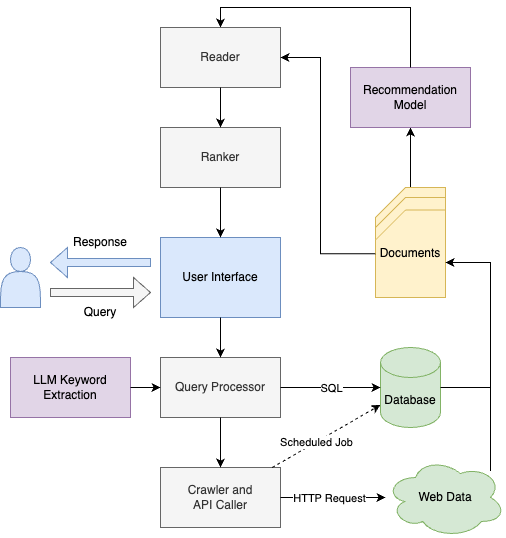
\includegraphics[width=1.0\linewidth]{doc//proposal//assets/sysarch.drawio.png}
    \caption{System Architecture}
    \label{fig:sysarch}
\end{figure}

\begin{enumerate}
    \item  {User Interface (UI)}: The user interface consists of a search box for the user to type queries and an area to display search results (response). Most of the major front-end web development frameworks can provide the components we need. It is proposed that we use HTML + CSS + JavaScript as the project’s UI solution. Additional libraries and dependencies may be introduced in the engineering process.

    \item {Query Processor}: The query processor processes user input. There are three main tasks for the query processor. First, it uses LLM for keyword extraction if necessary. When the user puts their question in a sentence, we need the help of LLM and tools like KeyBERT to extract the keyword from the query. Spelling correction and query expansion will be taken into consideration. Then it constructs SQL queries to search for keywords in the database for local data retrieval.

    \item {Crawler and API Caller}: The crawler and API caller will search for specific information for a movie entry, such as posters, and audience reviews. Wikipedia, for example, contains information about the plot and reception of the movie. Additionally, the crawler also runs regularly to update or insert entries to the database.

    \item {Recommendation Model}: The input of the recommendation model is proposed to be a particular movie entry. It returns other similar movie entries based on clustering. There are other ways to recommend movies, such as by returning movie guesses given a user profile or search history.

    \item {Reader}: Reader is a component where we gather all the relevant documents together and filter the repetitive documents. It passes 

    \item {Ranker}: Ranker uses algorithms based on term frequency and weighting to sort the results. Users can also choose different ranking mechanisms such as relevance or date.
\end{enumerate}

\section{Appendix}
This group consists of three members, Micah Harlan, Baiyi Zhang and Jianger Yu. Each team member will leverage there expertise to contribute to the completion of this project.The project is split into five sections. By 3/19/2024, the Data and Storage as well as API and Web Crawler, will be implemented. The subsequent steps LLM and Recommendation system should be implemented by 04/9/2024. The final step, User interface will be implemented by 5/7/2024, completing the application.

% references section
\bibliographystyle{IEEEtran}
\bibliography{IEEEabrv, proposal-ref}

\end{document}